\subsection{PULL (32)}

Request IPv4 addresses of other nodes in other to expand the neighbor table. 
This message can be sent to an existing neighbor or a DNL node. The number of 
addresses returned can be smaller than the number of addresses requested.

\begin{figure}[H]
    \centering
    \scalebox{.33}{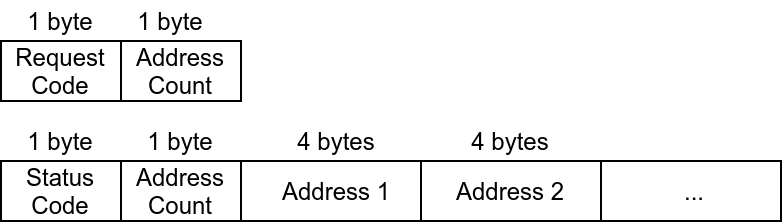
\includegraphics{figures/pull}}
\end{figure}

\subsection{PUSH (33)}

Sent by a node to make itself known to its new neighbors of which addresses 
were retrieved using the PULL message. The nodes which are receiving this 
message will add address of the message source to the neighbor table. Neither 
the request nor reply has additional data besides the request and status codes.

\subsection{BYE (34)}

Sent by a node to notify its neighbors and one of the DNL nodes that it will 
leave the network so they can remove the node from neighbor table and perform 
proper cleanup. The request does not have additional data besides the request 
code. There is no reply associated with the request.

\subsection{DEAD (35)}

Used to notify a node's neighbors and DNL nodes that some other nodes were 
found to be dead (not responding). These dead nodes did not send the BYE 
message before leaving (this may be due to a software crash or power failure). 
The nodes which are receiving this message should check if the nodes at the 
received messages are indeed dead by pinging before removing them from the 
neighbor table. The reply for this message does not have any data besides the 
status code.

\begin{figure}[H]
    \centering
    \scalebox{.33}{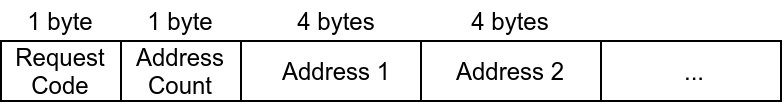
\includegraphics{figures/dead}}
\end{figure}

\subsection{PING (36)}

Used in conjunction with the DEAD message. Pings a node to confirm than it 
indeed left the network without sending the BYE message. Neither the request 
nor reply has additional data besides the request and status codes.

\subsection{DNLSYNC (37)}

This is a special message sent between DNL nodes to synchronize the distributed 
data structure. Updates are accumulated and periodically sent in bulk using a 
single message. The message data itself contains a list of entries, each 
representing an update. An entry contains the type of the action (0 for 
\textit{Add Address} and 1 for \textit{Remove Address}) , the address to be 
added or removed and the time point at which the action was originally 
performed. The timestamp is crucial for resolving potential conflicting updates 
- for example a DNL node informs the others that a peer has joined the network 
while another informs that it left instead.

\begin{figure}[H]
    \centering
    \scalebox{.33}{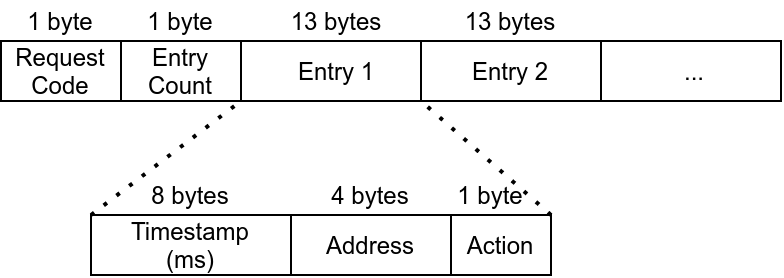
\includegraphics{figures/dnlsync}}
\end{figure}
